\section{Anhang}

\begin{table}[H]
	\centering
	\begin{tabular}{llrrrrrrr}
		\toprule
		{}         & Substanz    & M [g/mol] & Einwage [g] & $\Delta T$ & n [mol]  & $\Delta _c U_m$ [J/mol] & $\Delta _c U$ [J] & $C_{sys}$ [J] \\
		\midrule
		           & Benzoesäure & 122.12    & 0.512       & 0.904      & 0.004193 & -3.226e+06              & -13525.3          & -14873.14     \\
		           & Benzoesäure & 122.12    & 0.545       & 1.170      & 0.004463 & -3.226e+06              & -14397.0          & -12236.81     \\
		           & M           & 152.00    & 0.555       & 1.050      & 0.003651 & -3.897e+06              & -14232.7          &               \\
		           & M           & 152.00    & 0.576       & 1.161      & 0.003789 & -4.152e+06              & -15737.3          &               \\
		\midrule
		Mittelwert &             &           &             &            &          & -3.22e+06               &                   & -13554.97     \\
		           &             &           &             &            &          & -4.02e+06               &                   &               \\
		\bottomrule
  \end{tabular}
  \caption{Alle Ergebnisse und Messungen}
\end{table}

\begin{figure}[H]
	\includegraphics[width=\linewidth]{C:/Users/josefk/Desktop/kalorimetrie/src/img/Benzoesäure_1.PNG}
	\caption{Temperaturverlauf der 1. Probe}
\end{figure}

\begin{figure}[H]
	\includegraphics[width=\linewidth]{C:/Users/josefk/Desktop/kalorimetrie/src/img/Benzoesäure_2.PNG}
	\caption{Temperaturverlauf der 2. Probe}
\end{figure}

\begin{figure}[H]
	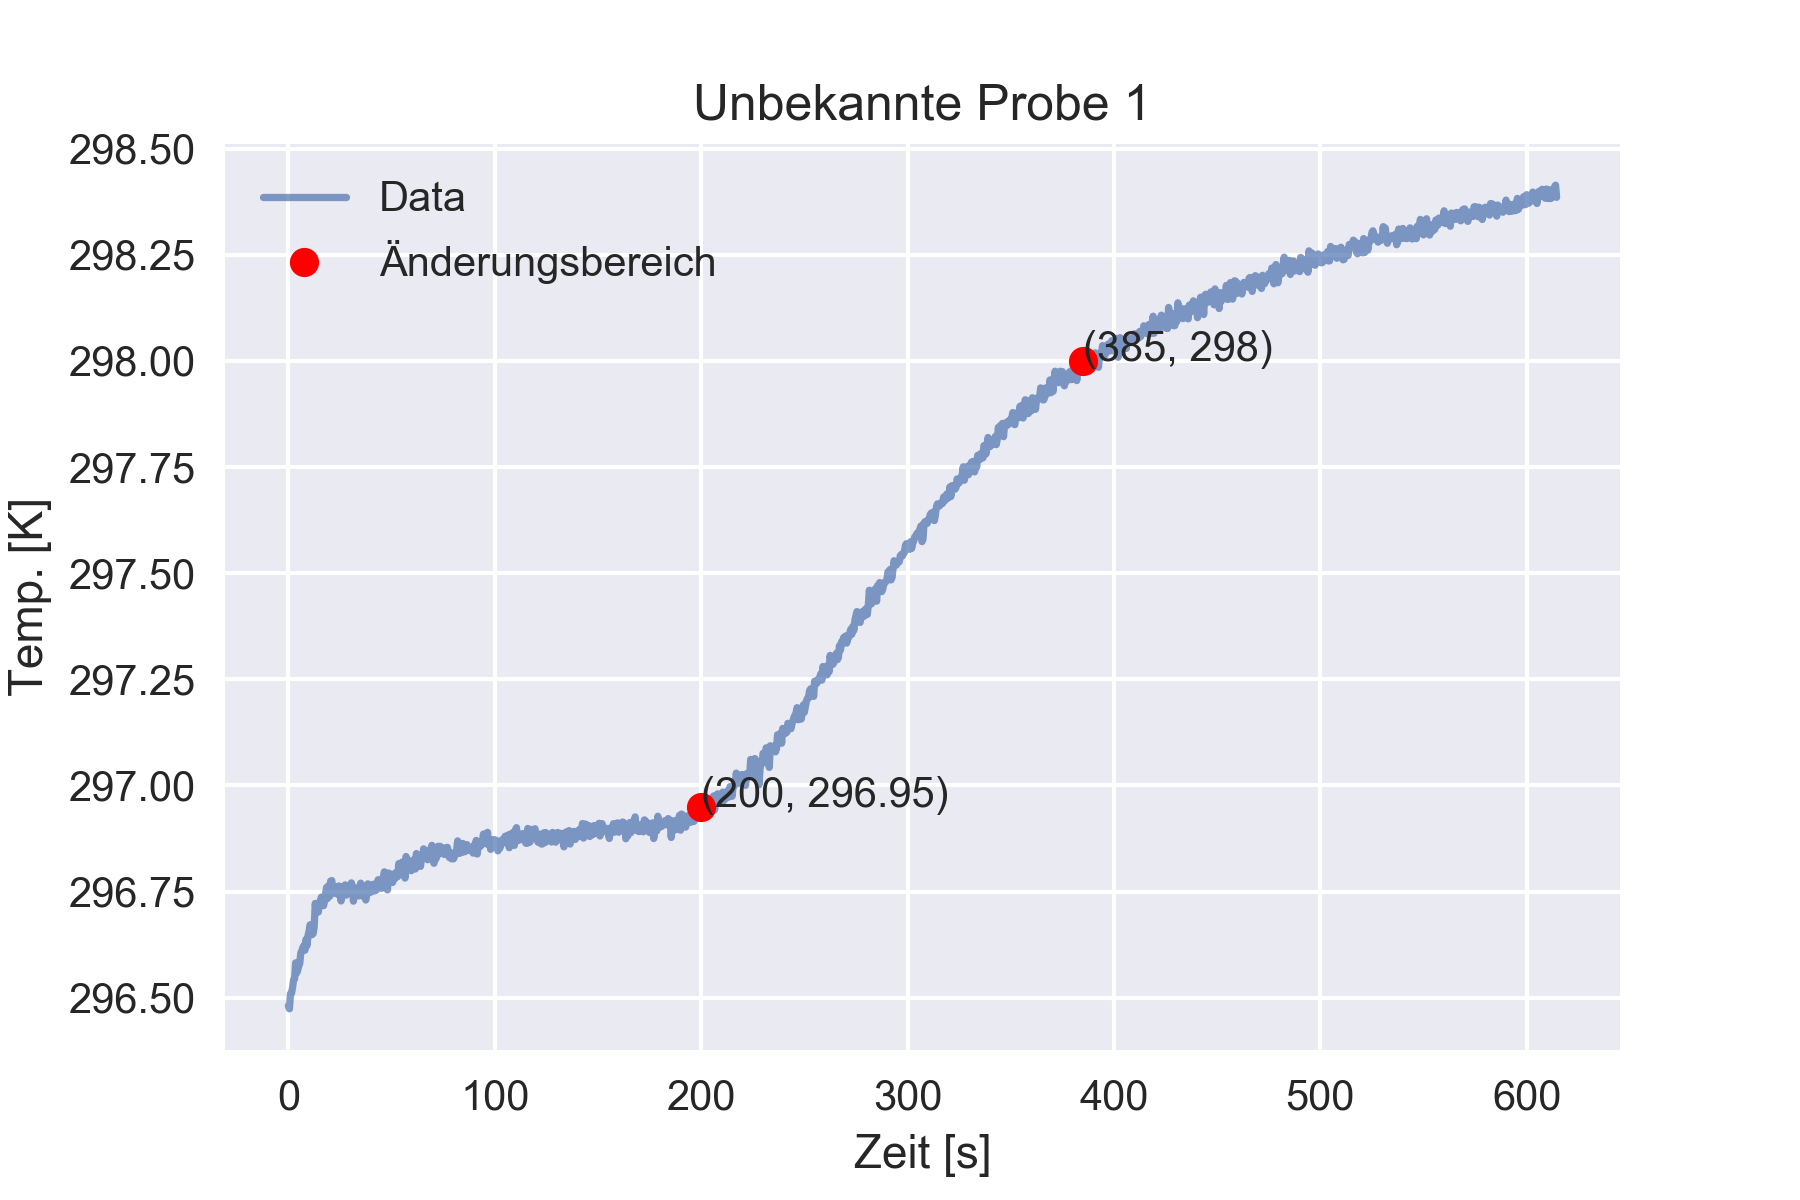
\includegraphics[width=\linewidth]{C:/Users/josefk/Desktop/kalorimetrie/src/img/unbekannteProbe_1.PNG}
	\caption{Temperaturverlauf der 2. Probe}
\end{figure}

\begin{figure}[H]
	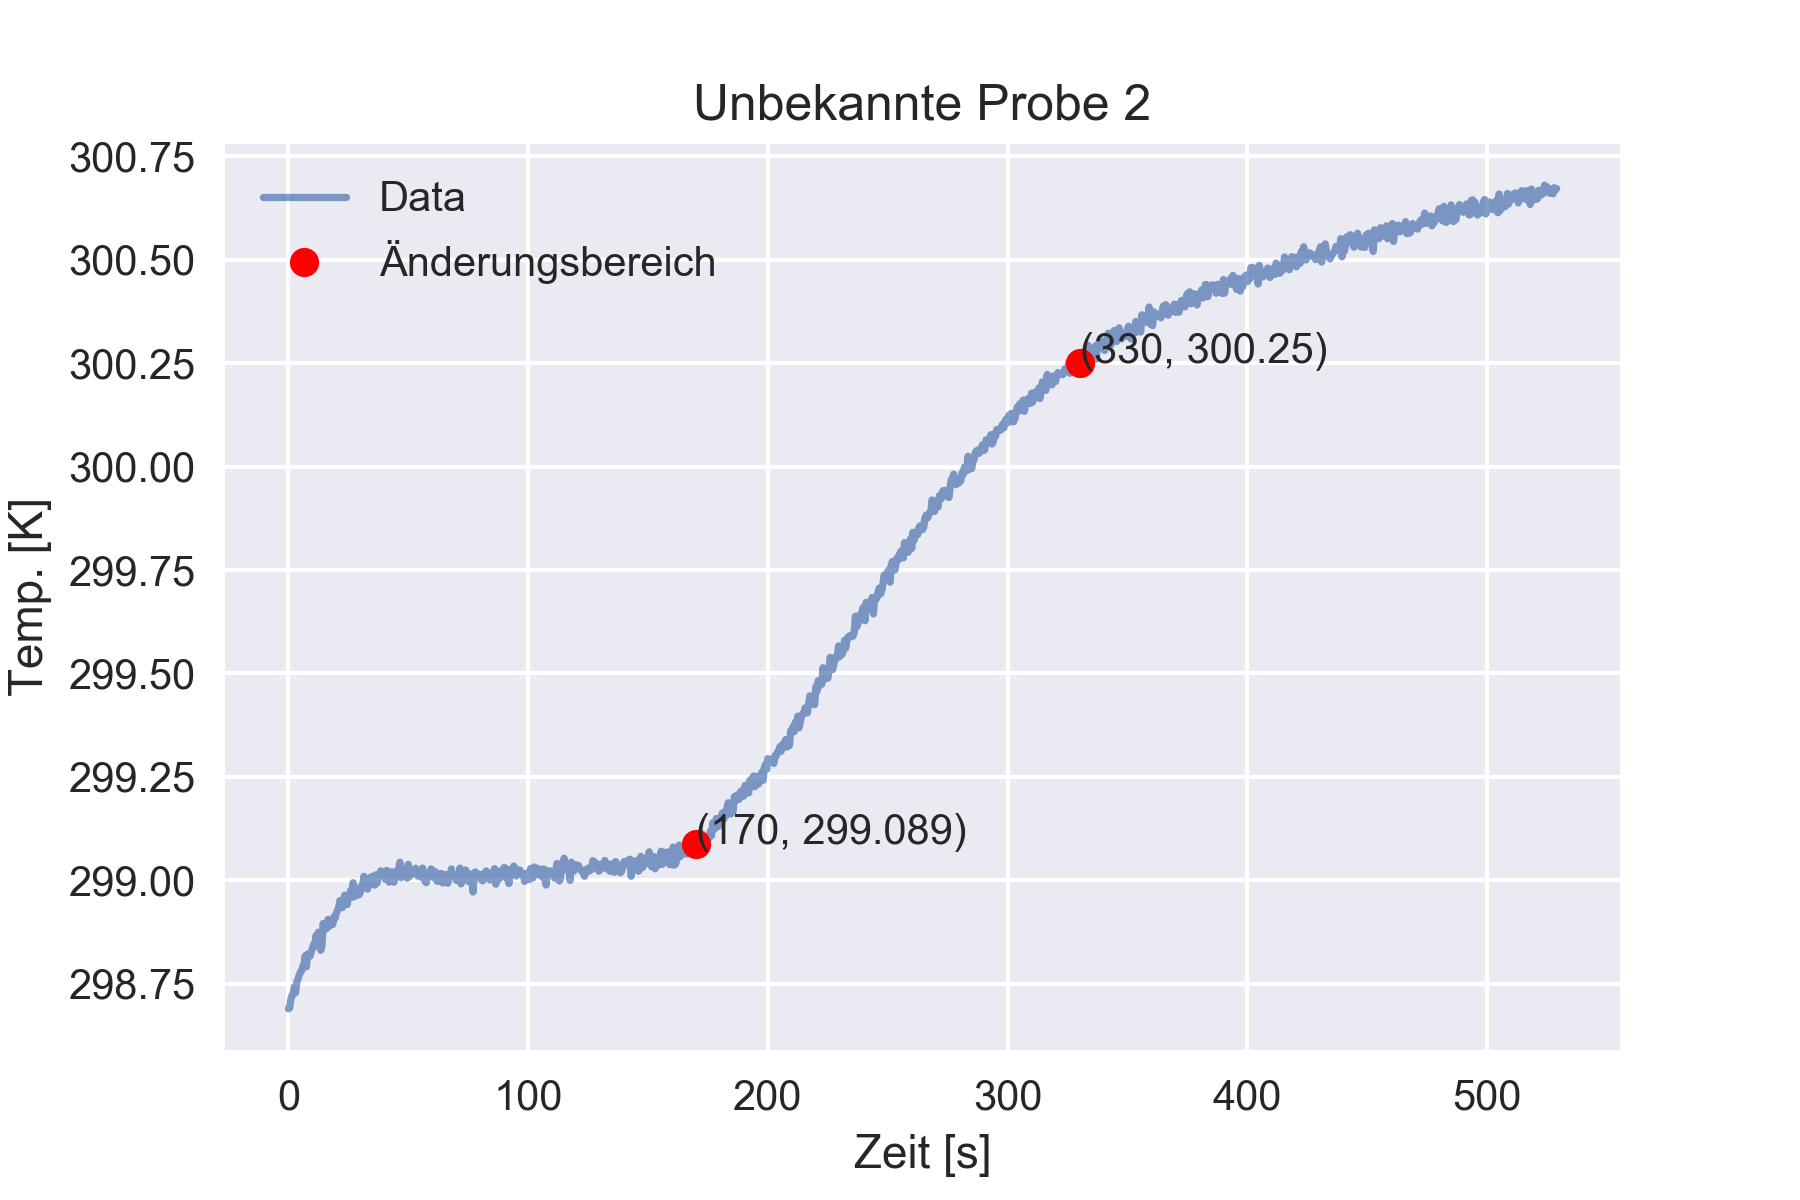
\includegraphics[width=\linewidth]{C:/Users/josefk/Desktop/kalorimetrie/src/img/unbekannteProbe_2.PNG}
	\caption{Temperaturverlauf der 2. Probe}
\end{figure}
